\begin{figure}[h]
    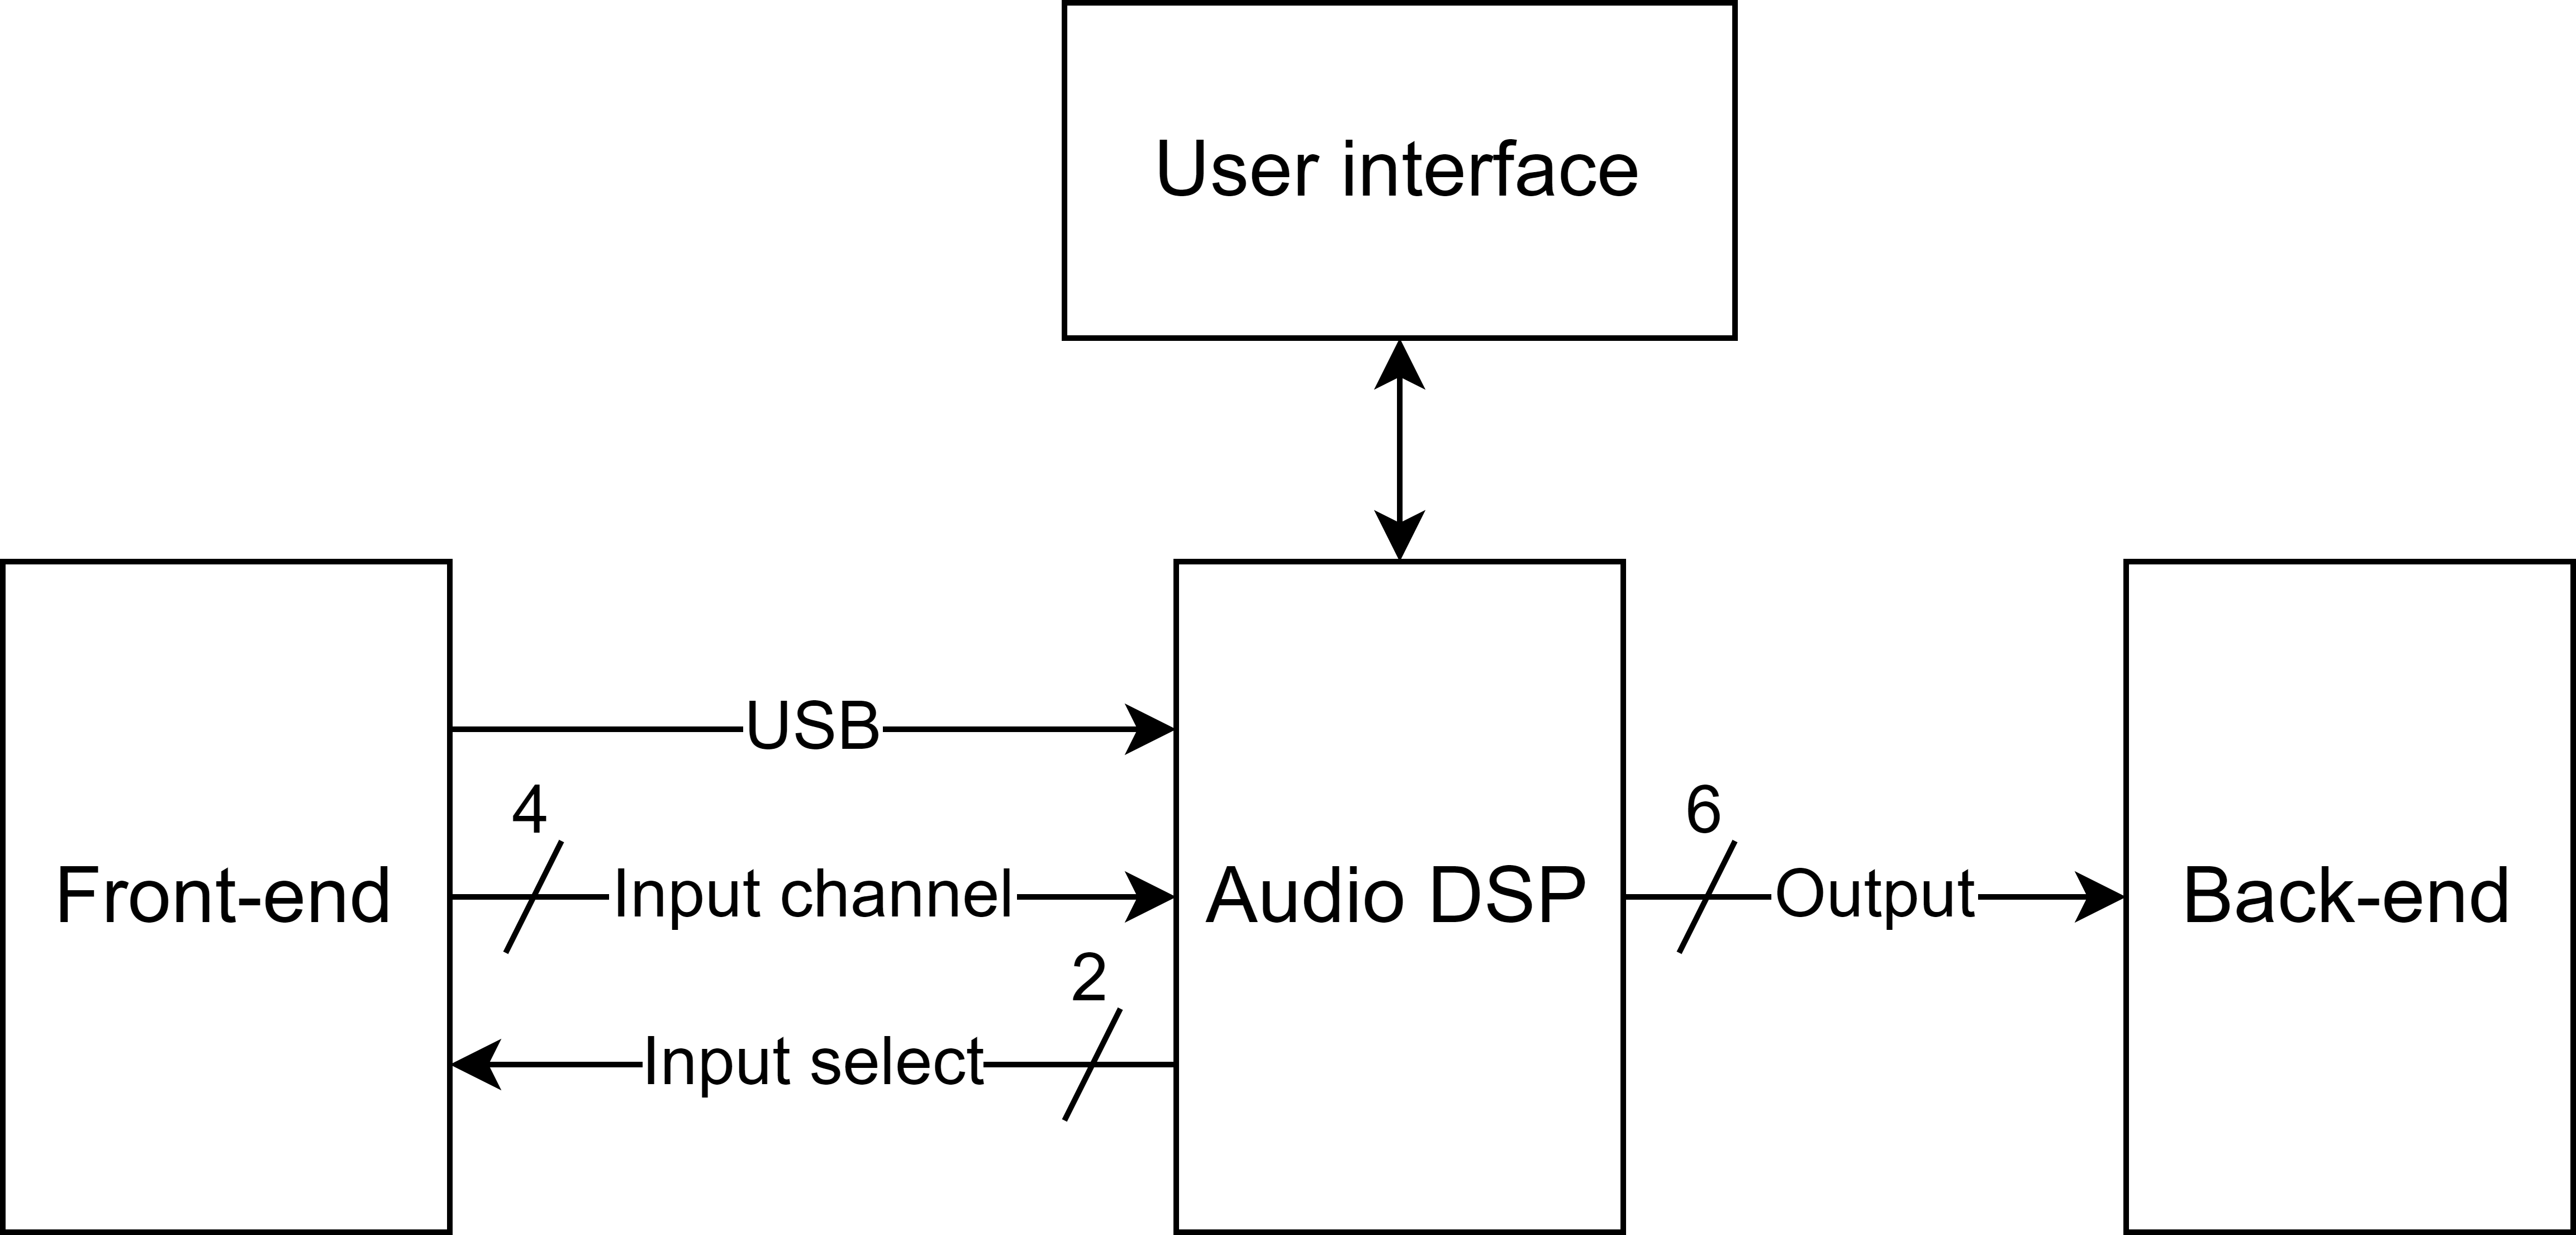
\includegraphics[width=\linewidth]{System context-top level.png}
    \caption{System context diagram of the top-level}
    \label{fig:sys-context-top}
\end{figure}

After the system requirement document has been aproved, the system context diagram could be made (see figure \ref*{fig:sys-context-top}).
The block called "Audio DSP" is the heart of the system.
This block represents the controller and thus the FPGA core.
This system context design diagram fulfills all the requirements, including the should and could haves.
Therefore the Audio-DSP has four analogue inputs, one USB input and six analogue outputs.
The input select line is for selecting what line input you want on input channel 1 and 2.
The user can either select a RCA or 6.35mm jack input on input channel 1 and 2.

With a user interface the user is able to configure the effect parameters, equalizer settings and volume of each channel.
The user is also able to rearrange the position of effects in the effects loop per channel.

\section{Front-end}
\begin{figure}[h]
    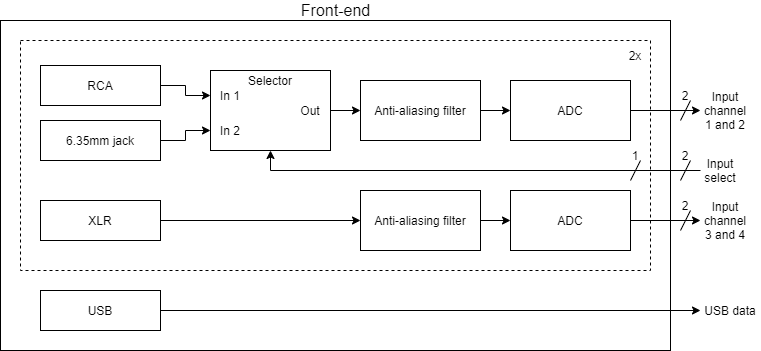
\includegraphics[width=\linewidth]{System context-front-end.png}
    \caption{System context diagram of front-end design}
    \label{fig:system-context-front-end}
\end{figure}

\section{Audio-DSP}
\begin{figure}[h]
    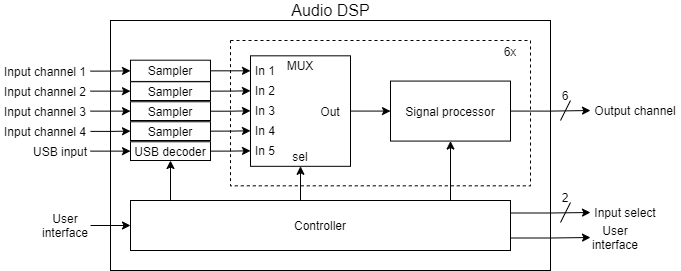
\includegraphics[width=\linewidth]{System context-audio DSP.png}
    \caption{System context diagram of Audio-DSP}
    \label{fig:sys-context-audio-dsp}
\end{figure}

The Audio-DSP block is made in the digital domain of the system (see figure \ref*{fig:sys-context-audio-dsp}). 
Therefore this block will be made in the FPGA. Each analogue input signal needs to be sampled in order for the system to be able to process the data. 
Thus each analogue input signal has a sampler block. The USB input signal has an USB decoder block as a sampler. 

After the sampler blocks each sampled signal goes to six channels with each a 5 to 1 MUX (multiplexer). 
With this MUX the user is able to select what input signal will be processed in each channel.
The chosen signal will then go to the signal processor block.
In the signal processor block the input signal will be modified by the various configurable effects, equalizer and volume settings.
These effects, equalizer and volume configurations can be configured by the user via the user interface.

After the signal has been modified by the signal processor block it will be fed out of the FPGA to the back-end of the system.

\section{Back-end}
\begin{figure}[h]
    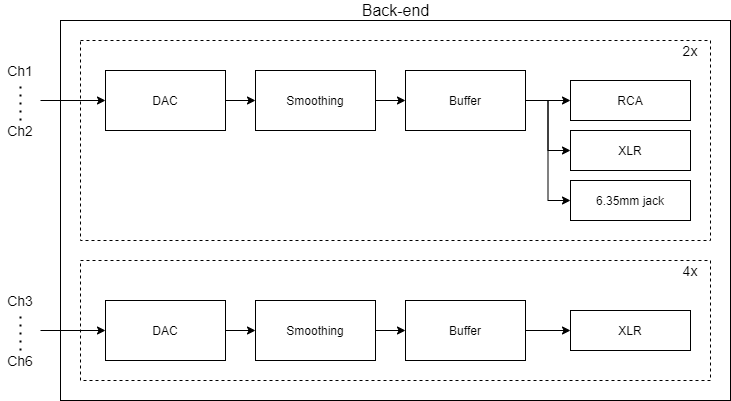
\includegraphics[width=\linewidth]{System context-back-end.png}
    \caption{System context diagram of back-end}
    \label{fig:system-context-back-end}
\end{figure}

\section{User interface}
